% -----------------------------*- LaTeX -*------------------------------
\documentclass[UTF8]{report}
% ------------------------------------------------------------------------
% Packages
% ------------------------------------------------------------------------
\usepackage{ctex} % 支持中文
\usepackage[body={7in, 9in},left=1in,right=1in]{geometry} % 改变页边距
\usepackage{amsmath} % AMS 的数学宏包
\usepackage{amsfonts} % AMS 的数学字体宏包
\usepackage{amssymb} % AMS 符号库
\usepackage{bm} % 数学公式中的黑斜体
\usepackage{amsthm} % AMS 的定理环境宏包
\usepackage{graphicx} % 插图
\usepackage{subfigure} % 插子图
\usepackage{nicefrac} % 好看的分数
\usepackage{mathrsfs} % mathscr font
\usepackage{caption} % caption
\usepackage{algorithm,algorithmicx} % 伪代码支持宏包
\usepackage[noend]{algpseudocode} % 伪代码
\usepackage{fancyhdr} % 设置页眉、页脚
\usepackage{adjustbox} % 图片尺寸自动调整
\usepackage{esint} % 积分符号
\usepackage{mathtools} % 数学宏包的重要补充
\usepackage{upgreek} % 数学环境的直立希腊字母
\usepackage{enumitem} % 使用enumitem宏包, 改变列表项的格式
\usepackage{color} % 支持彩色
\usepackage{extarrows} % 任意长度的箭头
\usepackage{tikz} % 绘图
\usepackage{xcolor} % 颜色宏包
\usepackage{breqn} % 公式自动换行
\usepackage{fontsize} % 字体大小
\usepackage[framemethod=TikZ]{mdframed} % 给文字加框
\usepackage{fontspec} % 字体库
\usepackage{bigstrut} % 用于表格中的换行
\usepackage{multirow} % 表格中多行单元格合并
\usepackage{rotating} % 旋转图形和表格      以上三者用于绘制三线表
\usepackage{booktabs} % 三线表宏包
\usepackage{scribe} % Scribe 模板
% ------------------------------------------------------------------------
% Macros
% ------------------------------------------------------------------------
%~~~~~~~~~~~~~~~
% Utility latin
%~~~~~~~~~~~~~~~
\newcommand{\ie}{\textit{i.e.}}
\newcommand{\eg}{\textit{e.g.}}
%~~~~~~~~~~~~~~~
% Environment shortcuts
%~~~~~~~~~~~~~~~
\newcommand{\balign}[1]{\ealign{\begin{align}#1\end{align}}}
\newcommand{\baligns}[1]{\ealigns{\begin{align*}#1\end{align*}}}
\newcommand{\bitemize}[1]{\eitemize{\begin{itemize}#1\end{itemize}}}
\newcommand{\benumerate}[1]{\eenumerate{\begin{enumerate}#1\end{enumerate}}}
%~~~~~~~~~~~~~~~
% Text with quads around it
%~~~~~~~~~~~~~~~
\newcommand{\qtext}[1]{\quad\text{#1}\quad}
%~~~~~~~~~~~~~~~
% Shorthand for math formatting
%~~~~~~~~~~~~~~~
\newcommand{\mbb}[1]{\mathbb{#1}}
\newcommand{\mbi}[1]{\boldsymbol{#1}} % Bold and italic (math bold italic)
\newcommand{\mbf}[1]{\mathbf{#1}}
\newcommand{\mc}[1]{\mathcal{#1}}
\newcommand{\mrm}[1]{\mathrm{#1}}
\newcommand{\tbf}[1]{\textbf{#1}}
\newcommand{\tsc}[1]{\textsc{#1}}
%\def\\langle {{\langle }}
%\def\\rangle {{\rangle }}
\newcommand{\sT}{\sf T}
\newcommand{\grad}{\nabla}
\newcommand{\Proj}{\Pi}
%~~~~~~~~~~~~~~~
% Common sets 定义数集符号
%~~~~~~~~~~~~~~~
\newcommand{\R}{\mathbb{R}}
\newcommand{\Z}{\mathbb{Z}}
\newcommand{\Q}{\mathbb{Q}}
\newcommand{\N}{\mathbb{N}}
\newcommand{\C}{\mathbb{C}}
\newcommand{\reals}{\mathbb{R}} % Real number symbol
\newcommand{\integers}{\mathbb{Z}} % Integer symbol
\newcommand{\rationals}{\mathbb{Q}} % Rational numbers
\newcommand{\naturals}{\mathbb{N}} % Natural numbers
\newcommand{\complex}{\mathbb{C}} % Complex numbers
%~~~~~~~~~~~~~~~
% Common functions
%~~~~~~~~~~~~~~~
\renewcommand{\exp}[1]{\operatorname{exp}\left(#1\right)} % Exponential
\newcommand{\indic}[1]{\mbb{I}\left(#1\right)} % Indicator function
\newcommand{\indicsub}[2]{\mbb{I}_{#2}\left(#1\right)} % Indicator function
\newcommand{\argmax}{\mathop\mathrm{arg\, max}} % Defining math symbols
\newcommand{\argmin}{\mathop\mathrm{arg\, min}}
\renewcommand{\arccos}{\mathop\mathrm{arccos}}
\newcommand{\dom}{\mathop\mathrm{dom}} % Domain
\newcommand{\range}{\mathop\mathrm{range}} % Range
\newcommand{\diag}{\mathop\mathrm{diag}}
\newcommand{\tr}{\mathop\mathrm{tr}}
\newcommand{\abs}{\mathop\mathrm{abs}}
\newcommand{\card}{\mathop\mathrm{card}}
\newcommand{\sign}{\mathop\mathrm{sign}}
\newcommand{\prox}{\mathrm{prox}} % prox
\newcommand{\rank}[1]{\mathrm{rank}(#1)}
\newcommand{\supp}[1]{\mathrm{supp}(#1)}
\newcommand{\norm}[1]{\lVert#1\rVert}
%~~~~~~~~~~~~~~~
% Common probability symbols
%~~~~~~~~~~~~~~~
\newcommand{\family}{\mathcal{P}} % probability family / statistical model
\newcommand{\iid}{\stackrel{\mathrm{iid}}{\sim}}
\newcommand{\ind}{\stackrel{\mathrm{ind}}{\sim}}
\newcommand{\E}{\mathbb{E}} % Expectation symbol
\newcommand{\Earg}[1]{\E\left[#1\right]}
\newcommand{\Esubarg}[2]{\E_{#1}\left[#2\right]}
\renewcommand{\P}{\mathbb{P}} % Probability symbol
\newcommand{\Parg}[1]{\P\left(#1\right)}
\newcommand{\Psubarg}[2]{\P_{#1}\left[#2\right]}
%\newcommand{\Cov}{\mrm{Cov}} % Covariance symbol
%\newcommand{\Covarg}[1]{\Cov\left[#1\right]}
%\newcommand{\Covsubarg}[2]{\Cov_{#1}\left[#2\right]}
%\newcommand{\model}{\mathcal{P}} % probability family / statistical model
%~~~~~~~~~~~~~~~
% Distributions
%~~~~~~~~~~~~~~~
%\newcommand{\Gsn}{\mathcal{N}}
%\newcommand{\Ber}{\textnormal{Ber}}
%\newcommand{\Bin}{\textnormal{Bin}}
%\newcommand{\Unif}{\textnormal{Unif}}
%\newcommand{\Mult}{\textnormal{Mult}}
%\newcommand{\NegMult}{\textnormal{NegMult}}
%\newcommand{\Dir}{\textnormal{Dir}}
%\newcommand{\Bet}{\textnormal{Beta}}
%\newcommand{\Gam}{\textnormal{Gamma}}
%\newcommand{\Poi}{\textnormal{Poi}}
%\newcommand{\HypGeo}{\textnormal{HypGeo}}
%\newcommand{\GEM}{\textnormal{GEM}}
%\newcommand{\BP}{\textnormal{BP}}
%\newcommand{\DP}{\textnormal{DP}}
%\newcommand{\BeP}{\textnormal{BeP}}
%\newcommand{\Exp}{\textnormal{Exp}}
%~~~~~~~~~~~~~~~
% Theorem-like environments
%~~~~~~~~~~~~~~~
%\theoremstyle{definition}
%\newtheorem{definition}{Definition}
%\newtheorem{example}{Example}
%\newtheorem{problem}{Problem}
%\newtheorem{lemma}{Lemma}
%~~~~~~~~~~~~~~~
% 组合数学的模板和作业里用到的一些宏包和自定义命令
%~~~~~~~~~~~~~~~
\renewcommand{\emph}[1]{\begin{kaishu}#1\end{kaishu}}
\newcommand{\falfac}[1]{^{\underline{#1}}}
\newcommand{\binomfrac}[2]{\frac{#1^{\underline{#2}}}{#2!}}
\newcommand{\ceil}[1]{\left\lceil #1 \right\rceil}
\newcommand{\floor}[1]{\left\lfloor #1 \right\rfloor}
\newcommand{\suminfty}[2]{\sum_{#1=#2}^{\infty}}
\newcommand{\suminftyk}[0]{\sum_{k=0}^{\infty}}
\newcommand{\sumint}[3]{\sum_{#1=#2}^{#3}}
\newcommand{\sumintk}[2]{\sum_{k=#1}^{#2}}
\newcommand{\suminti}[2]{\sum_{i=#1}^{#2}}
%~~~~~~~~~~~~~~~
% 定义新命令
%~~~~~~~~~~~~~~~
\newcommand*{\unit}[1]{\mathop{}\!\mathrm{#1}}
\newcommand*{\dif}{\mathop{}\!\mathrm{d}}%微分算子 d
\newcommand*{\pdif}{\mathop{}\!\partial}%偏微分算子
\newcommand*{\cdif}{\mathop{}\!\nabla}%协变导数、nabla 算子
\newcommand*{\laplace}{\mathop{}\!\Delta}%laplace 算子
\newcommand*{\deriv}[2]{\frac{\mathrm{d} #1}{\mathrm{d} {#2}}}
\newcommand*{\derivh}[3]{\frac{\mathrm{d}^{#1} #2}{\mathrm{d} {#3^{#1}}}}
\newcommand*{\pderiv}[2]{\frac{\partial #1}{\partial {#2}}}
\newcommand*{\pderivh}[3]{\frac{\partial^{#1} #2}{\partial {#3^{#1}}}}
\newcommand*{\dderiv}[2]{\dfrac{\mathrm{d} #1}{\mathrm{d} {#2}}}
\newcommand*{\dderivh}[3]{\dfrac{\mathrm{d}^{#1} #2}{\mathrm{d} {#3^{#1}}}}
\newcommand*{\dpderiv}[2]{\dfrac{\partial #1}{\partial {#2}}}
\newcommand*{\dpderivh}[3]{\dfrac{\partial^{#1} #2}{\partial {#3^{#1}}}}
\newcommand{\me}[1]{\mathrm{e}^{#1}}%e 指数
\newcommand{\mi}{\mathrm{i}}%虚数单位
%\newcommand{\mc}{\mathrm{c}}%光速 定义与mathcal冲突
\newcommand{\red}[1]{\textcolor{red}{#1}}
\newcommand{\blue}[1]{\textcolor{blue}{#1}}
%\newcommand{\Rome}[1]{\setcounter{rome}{#1}\Roman{rome}}
%~~~~~~~~~~~~~~~
% 公式环境中箭头符号的简写
%~~~~~~~~~~~~~~~
\newcommand{\ra}{\rightarrow}
\newcommand{\Ra}{\Rightarrow}
\newcommand{\la}{\leftarrow}
\newcommand{\La}{\Leftarrow}
\newcommand{\lra}{\leftrightarrow}
\newcommand{\Lra}{\Leftrightarrow}
\newcommand{\lgla}{\longleftarrow}
\newcommand{\Lgla}{\Longleftarrow}
\newcommand{\lgra}{\longrightarrow}
\newcommand{\Lgra}{\Longrightarrow}
\newcommand{\lglra}{\longleftrightarrow}
\newcommand{\Lglra}{\Longleftrightarrow}
%~~~~~~~~~~~~~~~
% 一些数学的环境设置
%~~~~~~~~~~~~~~~
%\newcounter{counter_exm}\setcounter{counter_exm}{1}
%\newcounter{counter_prb}\setcounter{counter_prb}{1}
%\newcounter{counter_thm}\setcounter{counter_thm}{1}
%\newcounter{counter_lma}\setcounter{counter_lma}{1}
%\newcounter{counter_dft}\setcounter{counter_dft}{1}
%\newcounter{counter_clm}\setcounter{counter_clm}{1}
%\newcounter{counter_cly}\setcounter{counter_cly}{1}
%\newtheorem{theorem}{{\hskip 1.7em \bf 定理}}
%\newtheorem{lemma}[theorem]{\hskip 1.7em 引理}
%\newtheorem{proposition}[theorem]{Proposition}
%\newtheorem{claim}[theorem]{\hskip 1.7em 命题}
%\newtheorem{corollary}[theorem]{\hskip 1.7em 推论}
%\newtheorem{definition}[theorem]{\hskip 1.7em 定义}
\newcommand{\problem}[1]{{\setlength{\parskip}{10pt}\noindent \bf{#1}}}
\newenvironment{solution}{{\noindent\hskip 2em \bf 解 \quad}}{}
\renewenvironment{proof}{{\setlength{\parskip}{7pt}\noindent\hskip 2em \bf 证明 \quad}}{\hfill$\qed$\par}
%\newenvironment{example}{{\noindent\hskip 2em \bf 例 \arabic{counter_exm}\quad}}{\addtocounter{counter_exm}{1}\par}
%\newenvironment{concept}[1]{{\bf #1\quad} \begin{kaishu}} {\end{kaishu}\par}
%~~~~~~~~~~~~~~~
% 本.tex文档中特殊定义命令
%~~~~~~~~~~~~~~~
\newcommand{\lno}[1]{\overline{#1}}
\newcommand{\NP}{\mathrm{NP}}
\newcommand{\coNP}{\mathrm{coNP}}
% \newcommand{\ISO}{\mathrm{ISO}}
\newcommand{\SAT}{\mathrm{SAT}}
\newcommand{\USAT}{\mathrm{USAT}}
% \newcommand{\threeSAT}{\mathrm{3\text{-}SAT}}
\renewcommand{\P}{\mathrm{P}}
% \mathchardef\mhyphen="2D
% \newcommand{\CNF}{\mathrm{CNF}}
% \newcommand{\DNF}{\mathrm{DNF}}
% \newcommand{\SetSp}{\mathrm{SET\text{-}SPLITTING}}
% \newcommand{\PUZZLE}{\mathrm{PUZZLE}}
% \newcommand{\SPATH}{\mathrm{SPATH}}
% \newcommand{\LPATH}{\mathrm{LPATH}}
% \newcommand{\UHAMPATH}{\mathrm{UHAMPATH}}
\newcommand{\SPACE}{\mathrm{SPACE}}
\newcommand{\NSPACE}{\mathrm{NSPACE}}
\newcommand{\PSPACE}{\mathrm{PSPACE}}
\newcommand{\NPSPACE}{\mathrm{NPSPACE}}
\newcommand{\DFA}{\mathrm{DFA}}
\newcommand{\NFA}{\mathrm{NFA}}
\newcommand{\TQBF}{\mathrm{TQBF}}
% \newcommand{\L}{\mathrm{L}}
\renewcommand{\O}{\mathrm{O}}
\newcommand{\NL}{\mathrm{NL}}
\newcommand{\coNL}{\mathrm{coNL}}
\newcommand{\LADDER}{\mathrm{LADDER_{DFA}}}
\newcommand{\hd}{\mathrm{\text{-}hard}}
\newcommand{\ADD}{\mathrm{ADD}}
\newcommand{\STCN}{\mathrm{STRONGLY\text{-}CONNECTED}}
\newcommand{\PATH}{\mathrm{PATH}}
\newcommand{\A}{\mathrm{A}}

% ----------------------------------------------------------------------
% Header information
% ------------------------------------------------------------------------

\begin{document}

\course{B0911005Y-01} 			%optional
\coursetitle{Introduction to Theory of Computation}	%optional
\semester{2023 Spring}		%optional
\lecturer{Mingji Xia}	%optional
\scribe{吉骏雄}		%required
\lecturenumber{8}			%required (must be a number)
\lecturedate{June 9}	%required (omit year)

\maketitle

% ----------------------------------------------------------------------
% Body of the document
% ------------------------------------------------------------------------


\textbf{第8.1次作业: 9.4, 9.5, 8.4, 8.6, 8.25. 选做: 9.12. 注: 书图9-5 $x_2$与其右下方的非门之间少连了一根导线.}

\problem{9.4} 如在图\ref{fig:9_4_1}中所做的那样, 标出图\ref{fig:9_4_2}所描绘的电路中所有门计算出的值, 从而说明它在输入$0110$上的计算历史. 
\begin{figure}[!htbp]
    \begin{minipage}[t]{0.49\linewidth}
        \centering
        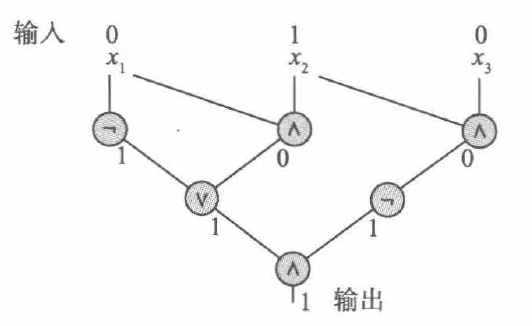
\includegraphics[width=7cm]{image/9.4.1.png}
        \caption{9.4题图1}
        \label{fig:9_4_1}
    \end{minipage}
    \begin{minipage}[t]{0.49\linewidth}
        \centering
        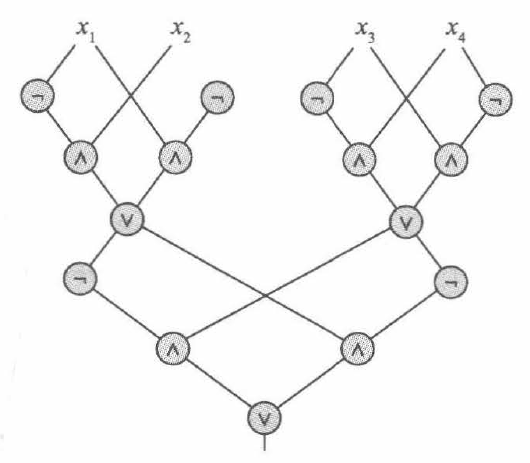
\includegraphics[width=7cm]{image/9.4.2.png}
        \caption{9.4题图2}
        \label{fig:9_4_2}
    \end{minipage}
\end{figure}

\begin{solution}
    结果如图\ref{fig:9_4_3}所示.
    \begin{figure}[!htbp]
        \centering
        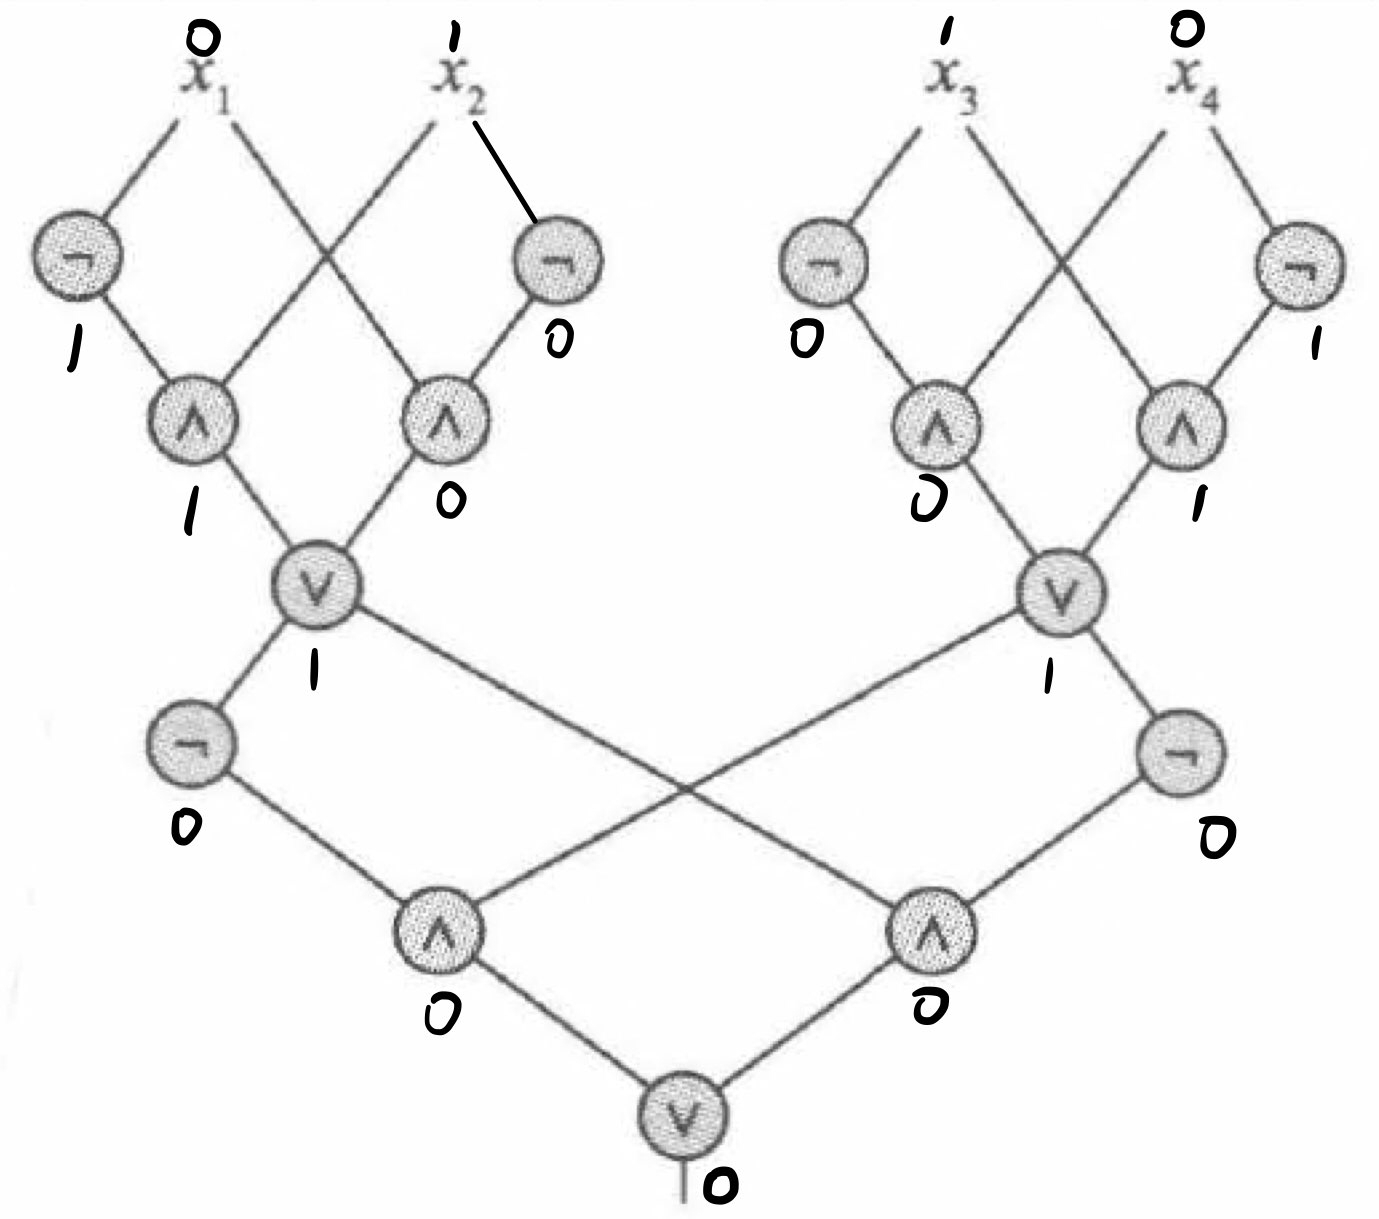
\includegraphics[width=7cm]{image/9.4.3.png}
        \caption{9.4题答案}
        \label{fig:9_4_3}
    \end{figure}
\end{solution}


\problem{9.5} 给出三个输入变量上计算奇偶函数的电路, 并说明它在输入$011$上的计算历史. 

\begin{solution}
    结果如图\ref{fig:9_5}所示.
    \begin{figure}[!htbp]
        \centering
        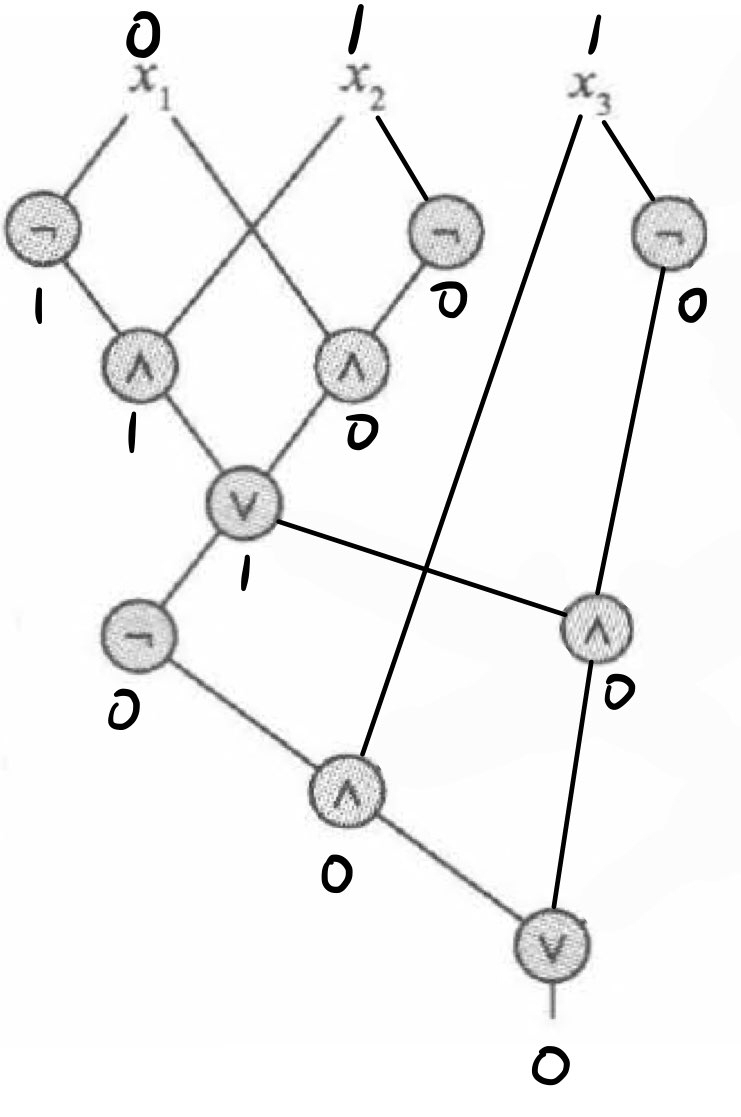
\includegraphics[width=4cm]{image/9.5.png}
        \caption{9.5题答案}
        \label{fig:9_5}
    \end{figure}
\end{solution}


\problem{8.4} 证明$\PSPACE$在并、补和星号运算下封闭. 

\begin{proof}
    \textbf{并运算:}

    $\forall L_1,L_2 \in \PSPACE$, 根据定义, 存在两个图灵机$M_1,M_2$分别能够判定$L_1,L_2$, 且所需空间$f_1(n), f_2(n)$均为多项式空间. 我们构造一个图灵机$M'$: $M' =$ ``对于输入$\omega$, 其中$\omega$是字符串:
    \begin{enumerate}
        \item 将输入复制一份在带上输入右面, 左面的原输入暂时封存, 用不会出现在$M_1, M_2$带字符表的符号将之分隔开.
        \item 使用右侧复制的内容, 模拟在输入$\omega$上运行$M_1$.
        \item 如果$M_1$接受, 则接受; 如果$M_1$拒绝, 则清空分隔符右侧的内容, 返回原输入状态.
        \item 模拟在输入$\omega$上运行$M_2$.
        \item 如果$M_2$接受, 则接受; 如果$M_2$拒绝, 则拒绝.
    \end{enumerate}
    ''

    可以看到, $M'$可能改写的格子数最多为$\max[f_1(|\omega|), f_2(|\omega|) + |\omega| + 1]$, 复杂多也是多项式级别的. $M'$能判定$L_1\cup L_2$, 因此$L_1\cup L_2 \in \PSPACE$. 因此$\PSPACE$在并运算下封闭.

    \textbf{星号运算:}

    设$M$能在 $O(n^a)$ 空间内判定 $L$. 我们构造一个图灵机$M'$: $M' =$ 对于输入 $\omega$, 其中$\omega = \omega_1 \omega_2 \omega_3\,...\,\omega_n$是字符串:
    \begin{enumerate}
        \item 若 $\omega = \varepsilon$, 则接受.
        \item 非确定地选择 $m, 1 \leq m \leq n$. 非确定地将 $\omega$ 分割为 $s_1s_2s_3\,...\,s_m$, 其中每个 $s_i$都非空.
        \item 对所有 $k=1 \sim m$:
        \item 在$M$上运行 $s_k$, 如果$M$拒绝, 则拒绝;
        \item 如果$M$接受, 则接受.
    \end{enumerate}
    

    可以看到, $M'$最多需要 $O(n)$ 的空间保存划分结果, 之后的运算都是多项式空间内可完成的. 因此$M'$能在多项式空间内判定$L^*$, 因此$L^* \in \PSPACE$. 因此$\PSPACE$在星号运算下封闭.

    \textbf{补运算:}

    $\forall L \in \PSPACE$, 根据定义, 存在图灵机$M$能够判定$L$, 且所需空间$f$为多项式空间. 我们构造一个图灵机$M'$, 其与$M$的区别仅为接受状态与拒绝状态互换, 即$q_{\mathrm{accept}}$与$q_{\mathrm{reject}}$互换. 这样构造的图灵机依然可以对任意输入停机, 所需的计算空间一致, 且接受的语言恰为$\overline{L}$. 因此$\PSPACE$在补运算下封闭.
\end{proof}


\problem{8.6} 证明$\PSPACE$难的语言也是$\NP$难的. 

\begin{proof}
    考虑两个特殊的语言: $\TQBF$以及$\SAT$, 以及分别识别这两个语言的两台图灵机$M_1, M_2$. 已经知道前者是一个$\PSPACE$完全的语言, 后者是一个$\NP$完全的语言. 我们证明$\TQBF$是$\NP$难的, 可以间接地证明$\SAT \leq_p \TQBF$, 存在一个多项式时间的图灵机$M$能够通过将$\SAT$多项式时间规约到$\TQBF$的方法识别它: $M =$ ``对于输入$\phi$, 其中$\phi$是一个布尔表达式:
    \begin{enumerate}
        \item 为输入的布尔表达式外侧添加一对括号.
        \item 检查输入的布尔表达式$\phi$中所有的变量, 为每个变量$x$在表达式前端添加一个对应的存在量词$\exists\,x$. 这样得到一个前束范式形式的全量词化的布尔表达式$\psi$, 输出之.
    \end{enumerate}
    ''
    接下来模拟在输入$\psi$上运行$M_2$ (能识别$\TQBF$的图灵机), 其接受与拒绝同 $M$ 的输入 ``是否在 $\SAT$中'' 的结果一致.

    由于除添加括号外, 操作次数等于变量数, 故该规约是多项式时间内的; 即可计算函数$f: \phi \rightarrowtail \psi$是多项式时间可计算函数. 因此得到$\SAT \leq_p \TQBF$.
    
    由于$\SAT$是$\NP$完全的, 因此$\forall L \in \NP\hd\,,\ \forall L' \in \PSPACE\hd$, 均有$L \leq_p \SAT \leq_p \TQBF \leq_p L' \Longrightarrow L \leq_p L'$, 故$\PSPACE$难的语言也是$\NP$难的. 
\end{proof}

\problem{8.25} 梯子(ladder) 是一个字符串的序列$s_1, s_2, \dots, s_k$, 其中每个字符串与前一个字符串恰好只在一个字母上不同. 例如, 下面是一个英文单词的梯子: 
\[
    \text{head, hear, near, fear, bear, beer, deer, deed, feed, feet, fret, free}
\]
令$\LADDER = \{ \langle M,s,t \rangle \mid M\text{ 是一个 } \DFA, L(M)\text{ 包含一个以字符串 }s\text{ 开头、以字符串 }t\text{ 结束的梯子 } \}$. 证明$\LADDER$属于$\PSPACE$. 

\begin{proof}
    根据Savitch定理, 我们有:
    \[
        \NSPACE(f(n)) \subseteq \SPACE(f^2(n))
    \]

    由于多项式的平方依旧是多项式, 所以:
    \[
        \NPSPACE = \bigcup_{i=0}^{\infty} \NSPACE(n^i) \subseteq \bigcup_{i=0}^{\infty} \SPACE(n^{2i}) = \PSPACE
    \]

    所以我们可以通过证明$\LADDER \in \NPSPACE$, 来证明题目中的$\LADDER \in \PSPACE$. 构造一个非确定型图灵机$M$, 其能够在多项式空间内判定$\LADDER$. $M =$ ``对于输入$\langle M,s,t \rangle$, 其中$M$是一个$\DFA$, $s,t$是字符串:
    \begin{enumerate}
        \item 在原输入的最末端添加一个数字$t = |\Sigma|^{|s|}$, 这表示了和$s$长度相同的字符串的总可能个数.
        \item 从$s$开始, 按照$M$的转移函数, 模拟$M$在输入$s$上的运行. 如果$M$在$s$上拒绝, 则拒绝.
        \item 如果$s$与$t$相同, 则接受.
        \item 非确定地选择$s$中的任意一个变量, 并非确定地 (即同时) 将其替换为$\Sigma$中的任意一个字母 (除了原本的字母以外), 并将其作为新的字符串, 覆写在原本$s$的位置上.
        \item 对$t$的值减去$1$.
        \item 如果$t=0$, 说明已经遍历过了所有可能性, 依旧没有抵达可以被接受的$t$, 则拒绝.
        \item 返回第$2$个步骤继续执行.
    \end{enumerate}
    ''

    可以发现, 空间使用不超过$f(n) = n + |s| + c + |s|\log |\Sigma|$, 其中$n$是输入字符串长度, $c$是分隔末尾添加数字所用的分隔符长度. 显然空间使用量是多项式的, 宽松估计也有$f(n) = \O(n^2)$. 因此$\LADDER \in \NPSPACE$, 从而$\LADDER \in \PSPACE$.
\end{proof}




\newpage

\textbf{第8.2次作业: 8.3, 8.1, 8.11(a), 8.33}

\problem{8.3} 考虑下图所示的广义地理学游戏, 其中起始结点就是由无源箭头指向的结点. 选手I有必胜策略吗?选手II呢?给出理由. 

\begin{figure}[!htbp]
    \centering
    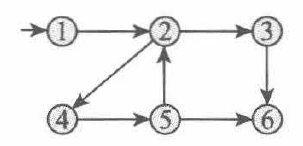
\includegraphics[width=7cm]{image/8.3.png}
    \caption{8.3题图}
    \label{fig:8_3}
\end{figure}

\begin{solution}
    选手II有必胜策略, 选手I没有.

    选手I第一步必须要从结点1前往结点2. 接下来, 选手II可以选择从结点2前往结点4. 之后, 选手I必须要从结点4前往结点5. 这时, 选手II只需选择从结点5前往结点6, 即可获得胜利, 因为结点6出度为$0$, 选手I无路可走.
\end{solution}


\problem{8.1} 证明对于任意函数$f: \N \rightarrow \R^+$, 其中$f(n) \geq n$, 不论用单带图灵机模型还是用双带只读输入图灵机模型, 所定义的空间复杂性类$\SPACE(f(n))$总是相同的. 

\begin{solution}
    需要证明两个命题: 单带图灵机模型定义的$\SPACE(f(n))$一定是双带只读输入图灵机模型定义的$\SPACE(f(n))$的子集, 反之亦然. 分别记录两种定义下的集合为$S_n$和$D_n$, 则需要证明$S_n \subseteq D_n$且$D_n \subseteq S_n$.

    \textbf{$S_n \subseteq D_n$:}

    $\forall L \in S_n$, 根据定义, 存在单带图灵机$M$能够判定$L$, 且所需空间$f$为多项式空间. 我们构造一个图灵机$M'$, 其与$M$的区别为: 将输入带改为只读输入带, 并在运行开始之后立即将只读输入带上的内容全部转写到读写工作带上; 之后$M'$完全在读写工作带上运行, 规则同$M$. 这样构造的图灵机依然可以对任意输入停机, 所需的计算空间完全一致, 且接受的语言恰为$L$. 因此$S_n \subseteq D_n$.

    \textbf{$D_n \subseteq S_n$:}

    $\forall L \in D_n$, 根据定义, 存在双带只读输入图灵机$M$能够判定$L$, 且所需空间$f$为多项式空间. 我们构造一个图灵机$M'$, 其与$M$的区别为: 将只读输入带和读写工作带合并成一条纸带, 只读输入只占有限长, 不变, 原读写工作带区域置于纸带上原只读输入带区域之后; 之后$M'$运行, 规则同$M$, 并以插入特殊字符的形式记录原两个读写头在原两条纸带上的位置. 这样构造的图灵机依然可以对任意输入停机, 所需的计算空间为$n + f(n) + \O(1) = \O(f(n))$ (比原本的计算空间多了一个除标记读写头外不可修改的输入字符串, 两带区域的分隔符, 以及标记原读写头位置的字符), 且接受的语言恰为$L$. 因此$D_n \subseteq S_n$.

    两个集合相互包含, 因此$S_n = D_n$, 即不论用单带图灵机模型还是用双带只读输入图灵机模型, 所定义的空间复杂性类$\SPACE(f(n))$总是相同的. 
\end{solution}


\problem{8.11(a)} 令$\ADD = \{ \langle x,y,z \rangle \mid x,y,z > 0 \text{ 且为二进制整数, } x + y = z\}$, 证明$\ADD \in L $. 

\begin{proof}
    我们构造一个双带只读输入图灵机$M$, 其能够在对数空间内判定$\ADD$. $M =$ ``对于输入$\langle x,y,z \rangle$, 其中$x,y,z$是二进制整数且均$>0$:
    \begin{enumerate}
        \item 仅用两位二进制数和一个整数进行读写工作带上的计算, 即带上始终只有两位与一个整数, 分别是进位$c$, 和位$s$, 位数$i$. 令$i=0$
        \item 考虑$x, y$的右数第$i$位$x_i,y_i$ ($i=0$代表的是最低位), 逐位将$x_i+y_i+c$记录到带上的$\overline{cs}$两bit位置处, 即求和后的$2$位二进制数替代了原本的数据.
        \item 如果$s \neq z_i$, 则拒绝. (以上, 若$x,y,z$中某一个数的位数不足, 则补充$0$).
        \item 如果$i \neq n$, 其中$n$为$x,y,z$三者最高位位数的最大值, 则将$i$加$1$, 回到第$2$步.
        \item 如果$c=0$, 则接受. 否则, 拒绝.
    \end{enumerate}
    ''

    可以发现, 空间使用不超过$f(n) = 2 + \log(n)$. 因此$\ADD \in L$.
\end{proof}


\problem{8.33} 设$A$是由正确嵌套的圆括号组成的语言. 例如, (())和(()(()))()属于$A$. 而)(则不属于$A$. 证明$A$属于$L$. 

\begin{proof}
    我们构造一个双带只读输入图灵机$M$, 其能够在对数空间内判定$\ADD$. $M =$ ``对于输入$\omega$, 其中$\omega$是圆括号组成的字符串:
    \begin{enumerate}
        \item 仅用一个整数进行读写工作带上的计算, 即带上始终只有一个整数$i$. 令$i=0$.
        \item 从左向右读取$\omega$的每一个字符, 如果是左括号, 则将$i$加$1$; 如果是右括号, 则将$i$减$1$; 进入下一步的判断.
        \item 如果$i < 0$, 则拒绝. 否则回到第二步继续读取下一个字符, 并进行相关操作.
        \item 读完所有字符之后, 如果$i = 0$, 则接受. 否则, 拒绝.
    \end{enumerate}
    ''

    可以发现, 空间使用不超过$f(n) = \log(n) + \O(1)$. 因此$\ADD \in L$.
\end{proof}

\newpage

\textbf{第8.3次作业:8.16,8.18,9.9,9.18}

\problem{8.16} 回忆一下,在有向图中,如果每一对结点间都有双向的有向路径连接,则它称为强连通的 (strongly connected)。令$\STCN = \{ \langle G \rangle \mid G \text{ 是强连通图 }\}$. 证明$\STCN$是$\NL$完全的。

\begin{proof}
    我们构造一个双带只读输入图灵机: $M =$ ``对于输入$\langle G \rangle$, 其中$G$是一个有向图:
    \begin{enumerate}
        \item 向工作带上写入两个数字$n, b, e, t, s$, 分别表示$G$的结点数, 以及当前正在遍历的结点编号 (编号不超过$n$). 令$b=e=1$.
        \item 从结点$b=1$开始, 遍历所有结点. 对于每一个结点, $e$又遍历所有结点. 对每一组结点对, 重复以下步骤:
        \item 如果$b=e$, 则跳过此次循环, 并回到第$2$步.
        \item 令$t=b$, $s=0$. 
        \item 非确定地选择一条以$t$为起点的边, 将$t$改为该边的终点. 如果不存在这样的边, 则拒绝. 如果$t$已经是$e$, 则回到第$2$步.
        \item $s$加$1$. 如果$s<n-1$, 则回到第$5$步. 否则, 所有可能简单路径都已经被某个分支尝试过, 则拒绝.
        \item 如果之前没被拒绝, 最终接受.
    \end{enumerate}
    ''

    可以发现, 空间使用不超过$f(n) = 5\log(n) + \O(1)$. 因此$\STCN \in \NL$.

    构造一个对数空间转换器$M$, 它能将$\PATH$映射到$\STCN$: $M =$ ``对于输入$\langle G, s, t \rangle$, 其中$G$是一个有向图:
    \begin{enumerate}
        \item 将$G$写至输出带上.
        \item 对于每一个结点$v$, 在输出带上添加一条从$v$指向$s$的边, 和一条从$t$指向$v$的边.
    \end{enumerate}
    ''

    只要$G$中有从$s$到$t$的路径, 那么$f(M)$就能被$\STCN$接受. 因此$\PATH \leq_L \STCN$.

    因此, $\STCN$是$\NL$完全的.
\end{proof}


\problem{8.18} 证明$\A_{\NFA}$是$\NL$完全的。

\begin{proof}
    我们构造一个双带只读输入图灵机: $M =$ ``对于输入$\langle N,\omega \rangle$, 其中$N$是一个$\NFA$, $\omega$是一个字符串:
    \begin{enumerate}
        \item 约定$\omega$从左向右数的的第$i$个字符为$\omega_i$.
        \item 选取初始状态$q_0$开始. 记录$i=0$于带上.
        \item 从$i \in \{1, 2, \dots , n\}$中, 非确定地选取一个状态$q_i$, 检查是否有$\delta(q_{i-1}, q_i) = \omega_i$ (注意, 此时空转移也算入其中). 如果不是, 则拒绝.
        \item 检查$q_n$是否为结束状态. 如果是, 则接受; 否则, 拒绝.
    \end{enumerate}
    ''

    可以发现, 空间使用不超过$f(n) = \log(n) + \O(1)$. 因此$A_{\NFA} \in \NL$.

    构造一个对数空间转换器$M$, 它能将$\PATH$映射到$\A_{\NFA}$: $M =$ ``对于输入$\langle G, s, t \rangle$, 其中$G$是一个有向图:
    \begin{enumerate}
        \item 将$G$中的每一个点写作一个状态, 写至输出带上.
        \item 将$G$中的每一条 (有向) 边写作一个转移函数, 写至输出带上, 其转移条件为任意一个字符.
        \item 将$|V|-1$个$1$作为输入$\omega$, 写至输出带上. 其中$|V|$为$G$的结点数.
    \end{enumerate}
    ''

    只要$G$中有从$s$到$t$的路径, 那么$f(M)$就能被$\A_{\NFA}$接受, 因为输入能让$\NFA$接受. 因此$\PATH \leq_L \A_{\NFA}$.

    因此, $\A_{\NFA}$是$\NL$完全的.
\end{proof}


\problem{9.9} 证明若$\NP = \P^{\SAT}$, 则$\NP = \coNP$

\begin{proof}
    假设$\NP = \P^{\SAT}$.

    $\forall L \in \P^{\SAT}$, 根据定义, 存在采用喻示$\SAT$的确定型喻示图灵机$M$能够判定$L$. 将$M$的接受状态与拒绝状态互换, 即$q_{\mathrm{accept}}$与$q_{\mathrm{reject}}$互换, 得到的图灵机$M'$; 由于$M'$是采用喻示$\SAT$的确定型喻示图灵机, 这样构造的图灵机依然可以对任意输入停机, 且所需的计算时间一致. $M'$接受的语言恰为$\overline{L}$, 所以$\overline{L} \in \P^{\SAT}$.

    因为$\forall L \in \coNP$, 均有$\overline{L} \in \NP$, 所以$\overline{L} \in \NP = P^{\SAT} \Longrightarrow L \in \P^{\SAT}$. 因此$\coNP \subseteq \P^{\SAT}$.

    因为$\forall L \in \P^{\SAT}$, 均有$\overline{L} \in \P^{\SAT} = \NP$, 所以$L \in \coNP$. 因此$\P^{\SAT} \subseteq \coNP$.

    综上, $\P^{\SAT} = \coNP$.
\end{proof}


\problem{9.18} 定义唯一满足 (unique-sat) 问题为: $\USAT = \{ \langle \phi \rangle \mid \phi \text{ 是一个只有唯一满足赋值的布尔公式 } \}$。证明$\USAT \in \P^{\SAT}$.

\begin{proof}
    我们构造一个非确定型图灵机$M$, 其能够在多项式时间内判定$\overline{\USAT}$. $M =$ ``对于输入$\phi$, 其中$\phi$是一个布尔公式:
    \begin{enumerate}
        \item 先仿照$\SAT$运行, 检查$\phi$是否可满足. 如果不能, 则接受.
        \item 非确定地选择两组赋值, 检查$\phi$在这两组赋值下是否都可满足. 如果是, 则接受. 如果否, 则拒绝.
    \end{enumerate}
    ''

    如果$\phi$不是唯一可满足的, 即$\phi \in \overline{\USAT}$, 那么$M$一定是两种情况之一: 不可满足的 (在第一步中被接受), 或者有两个不同的可满足赋值 (在第二步中被接受). 因此$M$能够判定$\overline{\USAT}$, 且只需要多项式时间 ($\SAT \in \NP$), 所以$\USAT \in \coNP \subseteq \P^{\SAT}$, 证毕.
\end{proof}



\textbf{第8.4次作业(书上均有答案,不需要提交):8.7,9.1-9.3}



\end{document}
